\section{Experiments}
\label{sec:exps}

%
% Corpus
%

\textcolor{red}{Describe all hyperparameters, including size of non-link minibatches}


We evaluated our models on several real world networks either directed or undirected. Theirs statistics and properties are summarized in table \ref{table:corpus}. The detailed descriptions are available in the online Koblenz network collection\footnote{http://konect.uni-koblenz.de/}.

\begin{table}[h]
\bgroup
\def\arraystretch{1} % 1 is the default, change whatever you need
	
\caption{Datasets networks used to train the models. Type A is for co-authorship, type C is for communication, type H is for hyperlinks, type L is for lexical network and I for interaction network.}

\resizebox{\textwidth}{!}{
\begin{tabular}{lrrrrcrrrr}
%\Xhline{2\arrayrulewidth}
\toprule
 Datasets     &   Nodes &   Edges &   Density & Directed  &    Diameter &   \multicolumn{3}{c}{Weights}  	& type     \\
 \cmidrule(l){7-9}  &   &   	  &   $\times 10^{-3}$		  & 		  &  		   	&  mean & std  & max             \\
%\hline
\midrule
astro-ph      & 16,706  & 121,251   & 0.87  & False & 14 & 1.8  & 3.3  & 306  & A  \\
%cond-mat     & 16,726  & 47,594    & 0.000 & False & 18 & 3.1  & 7.2  & 544  & A  \\
hep-th        & 8,361   & 15,751    & 0.45  & False & 1  & 5.2  & 16   & 1226 & A  \\
%netscience   & 1,589   & 2,742     & 0.002 & False & 2  & 2.2  & 1.9  & 33   & A  \\
moreno\_names & 1,773   & 9,131     & 5.81  & False & 8  & 1.8  & 3.0  & 100  & L  \\
manufacturing & 167     & 5,783     & 208   & True  & 3  & 14.3 & 44.9 & 1458 & C  \\
fb\_uc        & 1,899   & 20,296    & 5.63  & True  & 4  & 2.8  & 4.7  & 98   & C  \\
digg\_reply   & 30,398  & 85,247    & 0.09  & True  & 11 & 2.0  & 0.2  & 26   & C  \\
slashdot      & 51,083  & 130,370   & 0.05  & True  & 11 & 2.1  & 0.3  & 18   & C  \\
enron         & 87,273  & 320,154   & 0.04  & True  & 15 & 3.4  & 12.4 & 3904 & C  \\
wiki-link     & 100,312 & 887,426   & 0.09  & True  & 14 & 1.7  & 3.0  & 185  & H  \\
prosper-loans & 89,269  & 3,330,225 & 0.42  & True  & 2  & 2.0  & 0.2  & 16   & I  \\
%\Xhline{2\arrayrulewidth}
\bottomrule
\end{tabular}
}


\egroup
\label{table:corpus}
\end{table}


%
% Evaluaiton method (testing set and mesure)
%

For each run, we build a testset extracted from the original network composed of an equivalent number of edges and non-edges. We denote the ratio of the held-out edges by $t_{ratio}$. The evaluation of experiments were based on three metrics that we measured at a period of $5m$ minibatches until the stop criteria is met, where $m$ is the number of subsets of $S_0$ as defined in section \ref{sec:sampling}. For the stopping criteria we held-out a validation set with another 10 percent of the edges and same amount of non-edges from the training set. We stop the training when the average change on the log-likelihood on the validation is less than $0.001$ percent.

The gradient step parameters were set to $\tau=1024$ and $\kappa=0.5$ and the burn-in period  to $T_{burnin}=150$. For MMSB we set the hyper-parameters $\lambda_0=\lambda_1=0.1$ and for both MMSB and WMMSB we set the latent-class hyper-parameters to $\alpha_k=\frac{1}{K}$ and $K=10$.


%
% Perplexity
%

The most direct way to measure the convergence of the inference is the log-likelihood of the predictive distribution since the variational gradient optimizes a lower bound of this quantity. For a testset $\D_{test}$ the log-likelihood is

\begin{figure}[h]
\centering
	
\begin{subfigure}
     \centering
         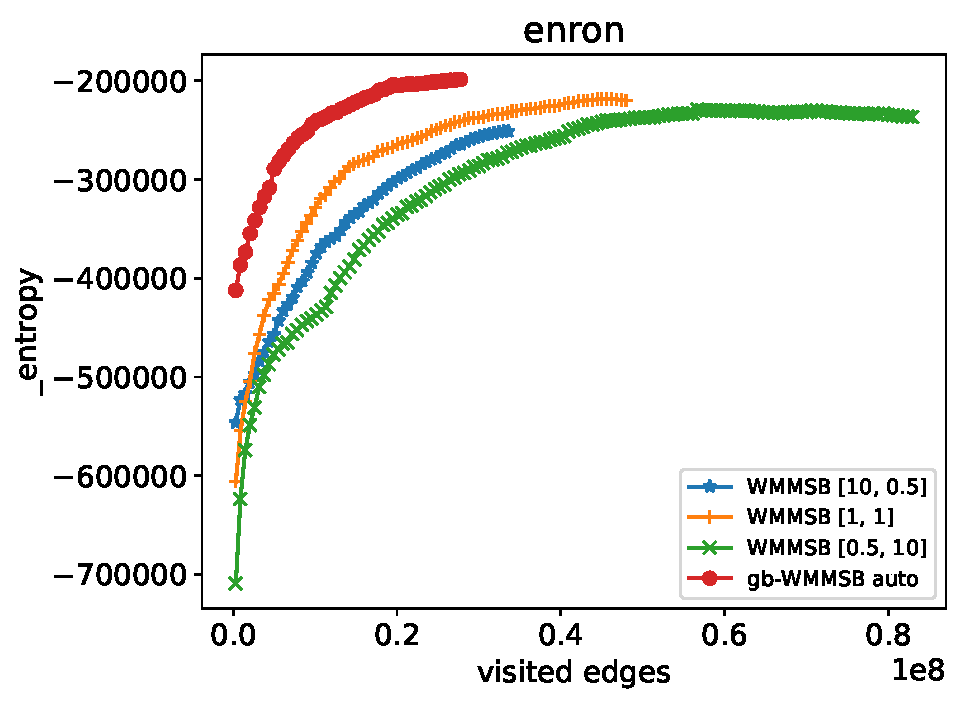
\includegraphics[width=0.32\textwidth]{warm2/enron_fig__entropy}
\end{subfigure}
\begin{subfigure}
         \centering
      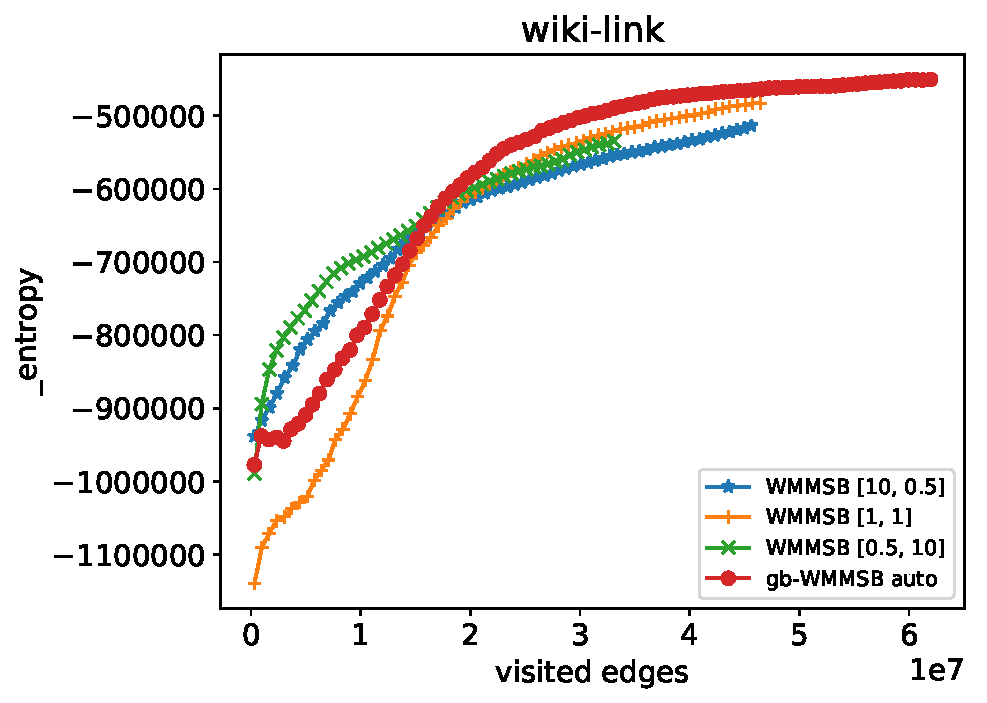
\includegraphics[width=0.32\textwidth]{warm2/wiki-link_fig__entropy}
\end{subfigure}
\begin{subfigure}
         \centering
      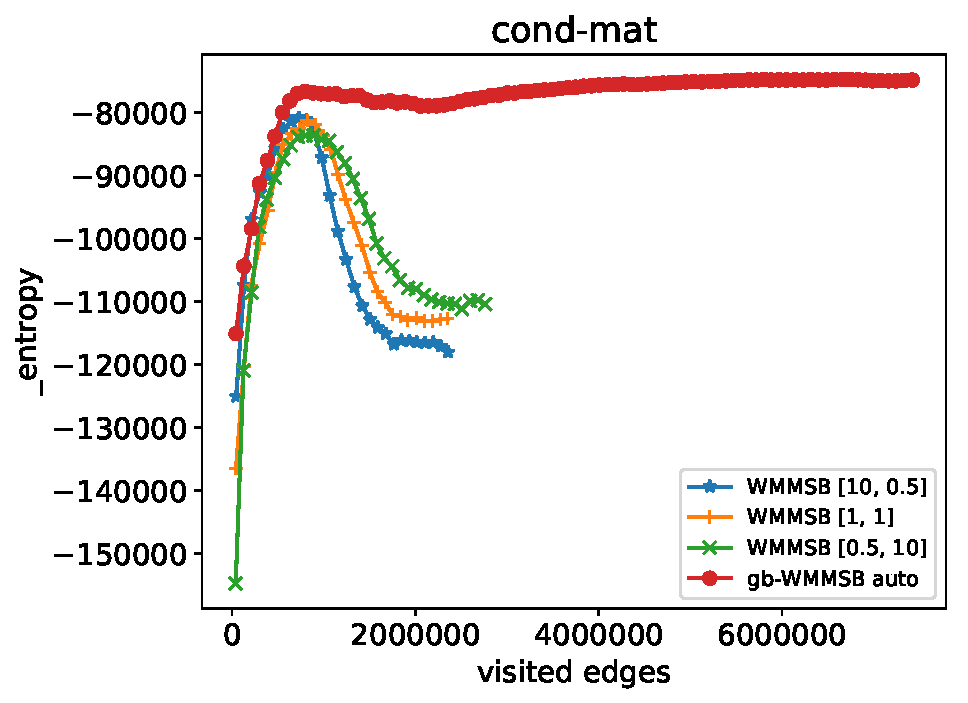
\includegraphics[width=0.32\textwidth]{warm2/cond-mat_fig__entropy}
\end{subfigure}
\caption{Log-likelihood convergence for WMMSB for different gamma prior. The bg-WMMSB model converges faster compared to fixed Gamma settings.}

    \label{fig:conv_entropy}
\end{figure}

\begin{equation*}
\log p(\D_{test}) = \sum_{i,j \in \D_{test}} \log p(y_{ij} | \phih_{kk'}) p(k|\thetah_i) p(k'|\thetah_j)
%\log p(\D_{test}) = \sum_{i,j \in \D_{test}} \log p(y_{ij} | \phih_{kk'}) p(k|\thetah_i) p(k'|\thetah_j)
\end{equation*}


%
% ROC
%

We evaluate the capacity of the models to predict missing links with the ROC-AUC curve on the testset. For the weighted models, the measure consists to evaluate to what extent they can reconstruct the topology of the network and to compare them with binary models. Thus, for the WMMSB models we compute the probability of observing a link as the probability to generate at least one edge count,

\begin{table}
\centering
	
\caption{AUC-ROC performance comparaison for two different size of testsets. In the top table, the testsets contains 20 percent of the edges. In the bottom table the testsets contains 80 percent of the edges. Score are averaged on 10 independants runs and for each run we randomly build the testsets that were held-out during the inference. For the SCVB inference, we fix the sampling parameter $m=50$.}

\begin{tabular}{llllll}
\toprule
$t_{ratio}=0.2$             &   MMSB &   WMMSB & bg-WMMSB      &    SBM &   WSBM \\
\midrule

 astro-ph                & 0.735 $\pm$ 0.018   & 0.717 $\pm$ 0.013    & 0.739 $\pm$ 0.004         & 0.676 $\pm$ 0.049 & 0.729 $\pm$ 0.062 \\
 cond-mat                & 0.675 $\pm$ 0.007   & 0.612 $\pm$ 0.019    & 0.662 $\pm$ 0.032         & 0.728 $\pm$ 0.045 & 0.752 $\pm$ 0.054 \\
 hep-th                  & 0.682 $\pm$ 0.008   & 0.659 $\pm$ 0.008    & 0.689 $\pm$ 0.009         & 0.672 $\pm$ 0.036 & 0.616 $\pm$ 0.036 \\
 netscience              & 0.684 $\pm$ 0.03    & 0.586 $\pm$ 0.04     & 0.724 $\pm$ 0.029         & 0.733 $\pm$ 0.077 & 0.774 $\pm$ 0.057 \\
 manufacturing           & 0.900 $\pm$ 0.003   & 0.884 $\pm$ 0.01     & 0.886 $\pm$ 0.006         & 0.876 $\pm$ 0.014 & 0.659 $\pm$ 0.052 \\
 fb\_uc                  & 0.820 $\pm$ 0.105   & 0.883 $\pm$ 0.004    & 0.871 $\pm$ 0.009         & 0.807 $\pm$ 0.019 & 0.662 $\pm$ 0.017 \\
 enron                   & 0.640 $\pm$ 0.159   & 0.849 $\pm$ 0.016    & 0.844 $\pm$ 0.021         & 0.562 $\pm$ 0.048 & 0.498 $\pm$ 0.088 \\
 wiki-link & 0.522 $\pm$ 0.12    & 0.723 $\pm$ 0.107    & 0.779 $\pm$ 0.016         & 0.615 $\pm$ 0.043 & 0.553 $\pm$ 0.047 \\

\bottomrule
\end{tabular}

\begin{tabular}{llllll}
\toprule
$t_{ratio}=0.8$             &   MMSB &   WMMSB & bg-WMMSB      &    SBM &   WSBM \\
\midrule

 astro-ph                & 0.729 $\pm$ 0.011   & 0.708 $\pm$ 0.008    & 0.739 $\pm$ 0.006         & 0.462 $\pm$ 0.046 & 0.617 $\pm$ 0.09  \\
 cond-mat                & 0.647 $\pm$ 0.01    & 0.601 $\pm$ 0.013    & 0.635 $\pm$ 0.015         & 0.474 $\pm$ 0.077 & 0.553 $\pm$ 0.04  \\
 hep-th                  & 0.652 $\pm$ 0.007   & 0.646 $\pm$ 0.004    & 0.631 $\pm$ 0.019         & 0.446 $\pm$ 0.053 & 0.457 $\pm$ 0.057 \\
 netscience              & 0.613 $\pm$ 0.011   & 0.580 $\pm$ 0.015    & 0.611 $\pm$ 0.018         & 0.470 $\pm$ 0.009 & 0.462 $\pm$ 0.013 \\
 manufacturing           & 0.883 $\pm$ 0.006   & 0.864 $\pm$ 0.008    & 0.851 $\pm$ 0.012         & 0.805 $\pm$ 0.023 & 0.654 $\pm$ 0.036 \\
 fb\_uc                  & 0.789 $\pm$ 0.104   & 0.857 $\pm$ 0.006    & 0.852 $\pm$ 0.011         & 0.569 $\pm$ 0.072 & 0.459 $\pm$ 0.083 \\
 enron                   & 0.659 $\pm$ 0.204   & 0.825 $\pm$ 0.075    & 0.866 $\pm$ 0.012         & 0.489 $\pm$ 0.108 & 0.344 $\pm$ 0.071 \\
 wiki-link & 0.608 $\pm$ 0.186   & 0.678 $\pm$ 0.12     & 0.779 $\pm$ 0.025         & 0.281 $\pm$ 0.053 & 0.227 $\pm$ 0.043 \\

\bottomrule
\end{tabular}


\label{table:roc}
\end{table}

\begin{equation*}
p(y_{ij} \geq 1 | \Thetah, \Phih) = 1 - \sum_{kk'} \thetah_{ik} \thetah_{jk'} e^{\phih_{kk'}}
\end{equation*}

The performance results in table \ref{table:roc} show that WMMSB is able to infer the topology of the networks. Furthermore, it outperforms the baseline for networks where weights represents natural information such as for communication and hyperlinks networks. 
In the other hand, MMSB and WMMSB under SCVI inference shows that they can infer the network topology when only observing a small portion of the networks, which represents an advantage in terms of scalability or when only a sub-graph of the real data are available.

%
% Sim
%

%For the weighted models, we further measure the capacity to predict right edge counts with a $l_1$ distance between the real count of the test set and the expected count of the models 
%
%\begin{equation*}
%D_{l_1}(D_{test} ||  \{\Thetah, \Phih\}) = \sum_{i,j \in \D_{test}} | y_{ij} - \E[y_{ij}|\Thetah, \Phih] |
%\end{equation*}



%
%  Figure analysis and commment
%




